\section{Resultados e discussão dos resultados}\label{sec:resultados}

Nesta sessão serão apresentados os resultados dos experimentos. Abaixo os gráficos de FMR/FNMR e BAcc para cada usuário, em ambos os conjuntos de dados utilizados.


\begin{figure}[H]
    \caption{}
    \label{fig:st_bacc_cmu}
    \centering
    \includegraphics[width=\textwidth]{Magalhães (CMU) - BAcc.png,}
\end{figure}
\begin{figure}[H]
    \caption{}
    \label{fig:st_bacc_keyrecs_1}
    \centering
    \includegraphics[width=\textwidth]{Magalhães (Keyrecs) - BAcc (Parte 1).png}              
\end{figure}
\begin{figure}[H]
    \caption{}
    \label{fig:st_bacc_keyrecs_2}
    \centering
    \includegraphics[width=\textwidth]{Magalhães (Keyrecs) - BAcc (Parte 2).png,}
\end{figure}
\begin{figure}[H]
    \caption{}
    \label{fig:st_global_bacc_cmu}
    \centering
    \includegraphics[width=\textwidth]{Magalhães com HPO global (CMU) - BAcc.png}
\end{figure}
\begin{figure}[H]
    \caption{}
    \label{fig:st_global_keyrecs_bacc_1}
    \centering
    \includegraphics[width=\textwidth]{Magalhães com HPO global (Keyrecs) - BAcc (Parte 1).png}
\end{figure}
\begin{figure}[H]
    \caption{}
    \label{fig:fig:st_global_keyrecs_bacc_2}
    \centering
    \includegraphics[width=\textwidth]{Magalhães com HPO global (Keyrecs) - BAcc (Parte 2).png}
\end{figure}
\begin{figure}[H]
    \caption{}
    \label{fig:st_user_cmu_bacc}
    \centering
    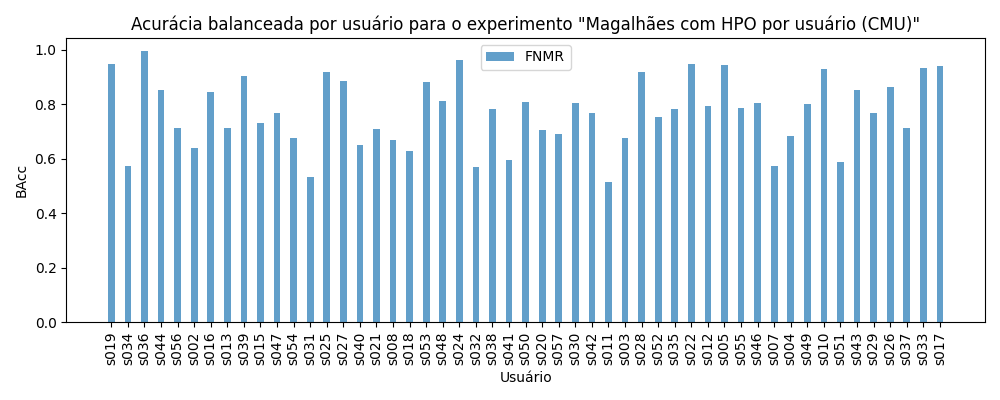
\includegraphics[width=\textwidth]{Magalhães com HPO por usuário (CMU) - BAcc.png}
\end{figure}
\begin{figure}[H]
    \caption{}
    \label{fig:st_user_keyrecs_bacc_1}
    \centering
    \includegraphics[width=\textwidth]{Magalhães com HPO por usuário (Keyrecs) - BAcc (Parte 1).png}
\end{figure}
\begin{figure}[H]
    \caption{}
    \label{fig:st_user_keyrecs_bacc_2}
    \centering
    \includegraphics[width=\textwidth]{Magalhães com HPO por usuário (Keyrecs) - BAcc (Parte 2).png}
\end{figure}
\begin{figure}[H]
    \caption{}
    \label{fig:rt_cmu_bacc}
    \centering
    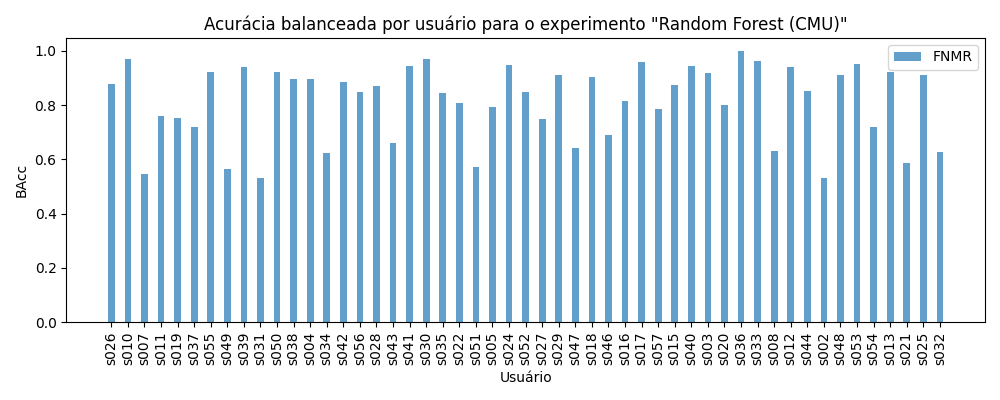
\includegraphics[width=\textwidth]{Random Forest (CMU) - BAcc.png}
\end{figure}
\begin{figure}[H]
    \caption{}
    \label{fig:svm_cmu_bacc}
    \centering
    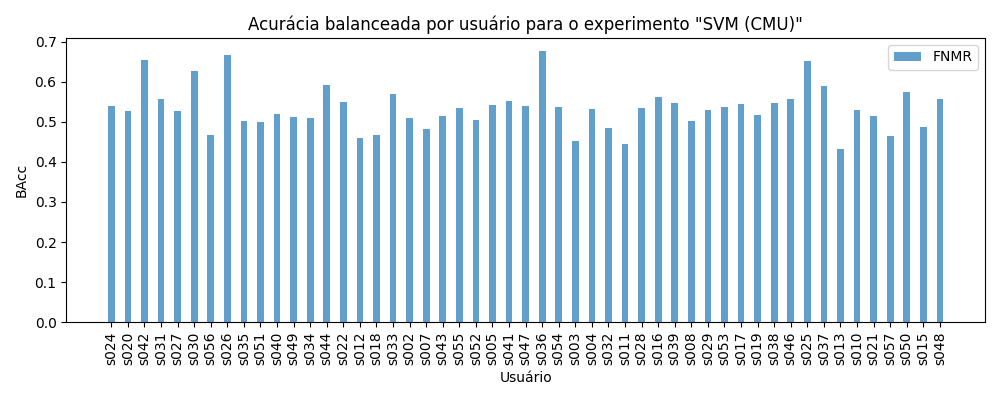
\includegraphics[width=\textwidth]{SVM (CMU) - BAcc.png}
\end{figure}
\begin{figure}[H]
    \caption{}
    \label{fig:svm_keyrecs_bacc_1}
    \centering
    \includegraphics[width=\textwidth]{SVM (Keyrecs) - BAcc (Parte 1).png}
\end{figure}
\begin{figure}[H]
    \caption{}
    \label{fig:svm_keyrecs_bacc_2}
    \centering
    \includegraphics[width=\textwidth]{SVM (Keyrecs) - BAcc (Parte 2).png}
\end{figure}
\begin{figure}[H]
    \caption{}
    \label{fig:svm_global_cmu_bacc}
    \centering
    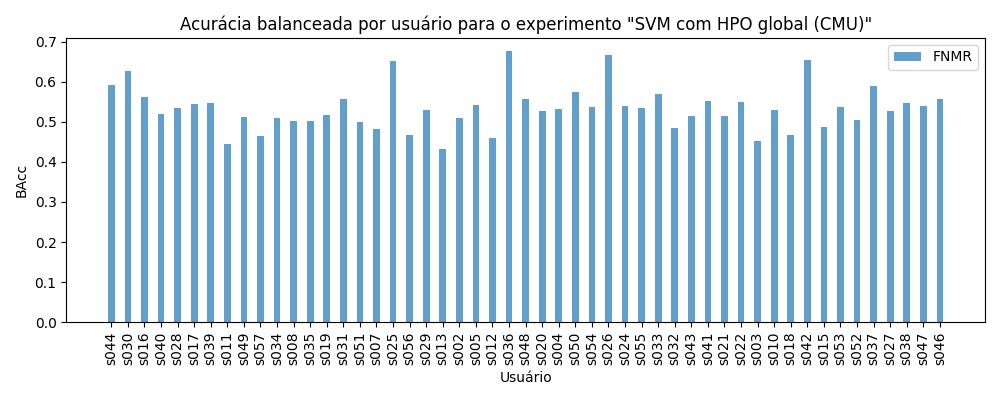
\includegraphics[width=\textwidth]{SVM com HPO global (CMU) - BAcc.png}
\end{figure}
\begin{figure}[H]
    \caption{}
    \label{fig:svm_global_keyrecs_bacc_1}
    \centering
    \includegraphics[width=\textwidth]{SVM com HPO global (Keyrecs) - BAcc (Parte 1).png}  
\end{figure}
\begin{figure}[H]
    \caption{}
    \label{fig:svm_global_keyrecs_bacc_2}
    \centering
    \includegraphics[width=\textwidth]{SVM com HPO global (Keyrecs) - BAcc (Parte 2).png}
\end{figure}
\begin{figure}[H]
    \caption{}
    \label{fig:svm_user_cmu_bacc}
    \centering
    \includegraphics[width=\textwidth]{SVM com HPO por usuário (CMU) - BAcc.png}
\end{figure}
\begin{figure}[H]
    \caption{}
    \label{fig:svm_user_keyrecs_bacc_1}
    \centering
    \includegraphics[width=\textwidth]{SVM com HPO por usuário (Keyrecs) - BAcc (Parte 1).png}
\end{figure}
\begin{figure}[H]
    \caption{}
    \label{fig:svm_user_keyrecs_bacc_2}
    \centering
    \includegraphics[width=\textwidth]{SVM com HPO por usuário (Keyrecs) - BAcc (Parte 2).png}
\end{figure}